%% This document gives an example on how to use the ntnubachelorthesis
%% LaTeX document class.
%% Use oneside for PDF delivery and twoside for printing in a book style
%% use language english, norsk, nynorsk and one of the following shortenings
%%  ``BSP'' Bachelor i Spillprogrammering,\\
%%  ``BRD'' Bachelor i drift av nettverk og datasystemer,\\
%%  ``BIS'' Bachelor i Informasjonssikkerhet,\\
%%  ``BPU'' Bachelor i Programvareutvikling, \\
%%  ``BIND'' Bachelor i Ingeniorfad - data, \\
%%  ``BADR'' Bachelor i drift av datasystemer, \\
%%  ``BIT'' Bachelor i informatikk, \\
%%  ``BABED'' Bachelor i IT-støttet bedriftsutvikling.
%%   for example \documentclass[BIS,norsk,twoside]{ntnuthesis/ntnubachelorthesis}

\documentclass[BSP,english,oneside]{ntnuthesis/ntnubachelorthesis}

\usepackage{csvsimple}
\usepackage{booktabs}
\usepackage{minted}
\usepackage{pdfpages}
\usepackage{enumerate}

\newcommand{\comment}[1]{\textcolor{blue}{\emph{#1}}}  %% use of the colour and you can see how to use commands with parts \comment{so what}

%% The class files defines these two
%% \newcommand{\NTNU}{Norwegian University for Science and Technology} %

% you can create you one #define like structures using the \newcommand feature
% you can change behaviour using \renewcommand

\newcommand{\com}[1]{{\color{red}#1}} % supervisor comment
%\renewcommand{\com}[1]{} %remove starting % to remove supervisor comments
% This will appear in text \com{Lecuters comment} and be visible unless you uncomment
% the renewcommand line.

\newcommand{\todo}[1]{{\color{green}#1}} % items to do
%\renewcommand{\todo}[1]{} %remove starting % to remove items to do

\newcommand{\n}[1]{{\color{blue}#1}} % other comment
%\renewcommand{\n}[1]{} %remove starting % to remove notes

\newcommand{\dn}[1]{} % add the d to a note to say that you have finished with it.


% Norwegian Characters,  needs the {} or to be separate from the next letters
% \o{}   \aa{}   \ae{}   so at the end of a word you can use \o  \aa   \ae
% \O{}   \AA{}   \AE{}   you can also just leave a space and latex will remove it
%    eg, NTNU i Gj\o vik  or NTNU i Gj\o{}vik

\begin{document}

\thesistitle{Conductor Hero - Project Report}
%\thesisshorttitle{} % use this if you have a very long title and want something shorter on the header pages
\thesisauthor{Rikhart Vigdal Bekkevold} %thesisauthorA, B, C etc
\thesisauthorA{Sabina Niewiadomska}
\thesisauthorB{Per-Morten Straume}
\thesisauthorC{Ida Ellinor Syverinsen}
\thesisauthorD{Andreas Wang}
\thesisauthorE{Yijie Zhou}

\nmtkeywords{Project Report, Virtual Reality, SteamVR, Unity Engine, ~Interaction Design, Game Design, 3D Modelling}

% Note: this can only be one paragraph with this template
\nmtdesc{
Experts in Teamwork is a course where students from various disciplines are put together in a team to work on a project throughout the semester. For the course, our group worked on a VR game called Conductor Hero where the player takes the role of a Conductor in a fantasy environment. The development of this project has taught us the importance of working with tight schedules as well as provided experience with cross disciplinary teams. The project report for Conductor Hero contains the technical details and methods for how the game was developed as well as discussions around the decisions that led to the final product. 
}


\nmtoppdragsgiver{\NTNU}
% TODO: Maybe this should be replaced by Sabina since she is PR
\nmtcontact{Andreas Wang, andrwan@stud.ntnu.no, 48048162}

\thesisdate{\ntnubachelorthesisdate}
\useyear{04.05.2018}

\nmtappnumber{1} %number of appendixes
\nmtpagecount{} %currently auto calculated but might be wrong % this is the file which contains all the details about your thesis

\makefrontpages % make the frontpages

\tableofcontents
\listoffigures
%\listoftables
%\listoflistings

\chapter{Introduction}
\chapter{Methods} \label{chap:methods}
\section{Idea Generation} 
The idea generation followed a ''divergent - emergent - convergent'' process~\cite{gameBook}, as shown in Figure~\ref{fig:ideaGeneration}. At the first stage, we conducted a brainstorming session, where each group member freely expressed their ideas related to VR and AR in the field of games, health or education. A range of ideas was generated, including a rehearsal room for musicians or dancing classes, a public speaking practice place, collaborative painting or sand painting, a virtual memory palace, a 3D-data visualisation room and simulators for activities like gardening, parachuting or car racing. 

After discussing all ideas we decided to apply dot-voting~\cite{gameBook} which helped us to prioritize our favourite ideas. All of us received three votes and we were asked to distribute the votes (dots) as we saw fit. This meant that we could put all three dots on one of the ideas or we could put one dot on three different ideas instead. When everyone had placed all their dots, we narrowed our focus to the three ideas with the most votes. 

One of the ideas was to create a service which lets the musicians or DJs play their own music and artists to display visualisations, while an audience could meet in virtual space to experience the audio-visual performance and dance together. Another was an educational chemistry game, aimed at school children. The final idea was to create an orchestral conducting game.

\begin{figure}[tbph]
    \centering
    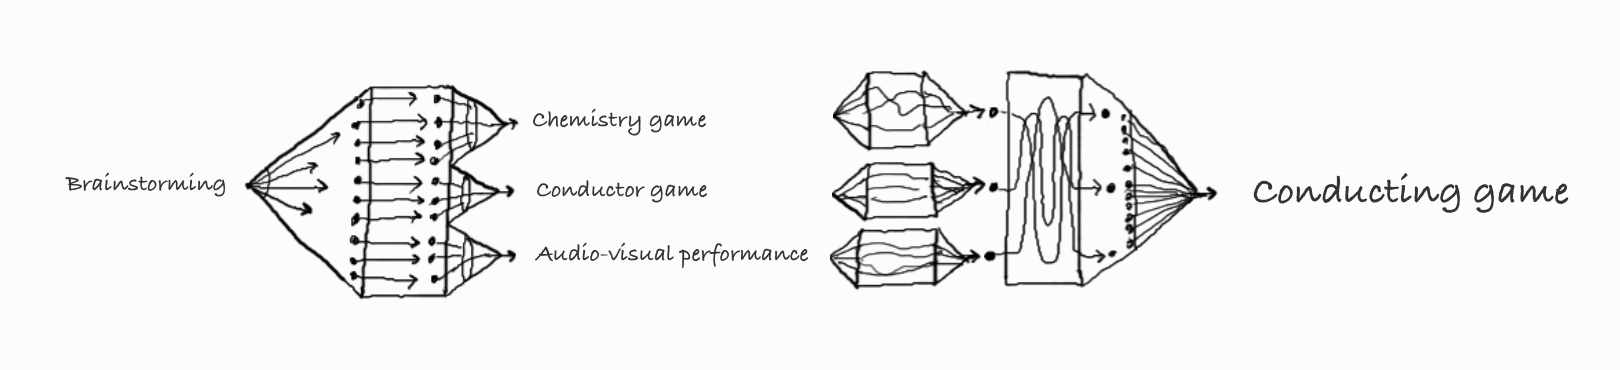
\includegraphics[width=1.0\textwidth]{images/ideaGenerationProcess.png}
    \caption[Idea Generation Process]{The process of idea generation~\cite{gameBook}}
    \label{fig:ideaGeneration}
\end{figure}

In the following discussion of these ideas, we sketched the scenarios of the games, as well as the implementation details. We now had a better feel for, and understanding of, each idea. Together we decided that we would like to try to develop the orchestra conductor game. Among the reasons for this choice was the strong musical background of four group members, as we believed our musical experience would help us to create a more interesting game scenario. The lack of market competitors also played a part in our decision, additionally, the VR technology seemed to suit conducting well. Sketching of ideas was further used in the project to illustrate our ideas to each other as shown in Figure~\ref{fig:tablesketch} which contains a sketch of how we envisioned the various elements of the Conductor Table. 

\begin{figure}[tbph]
    \centering
    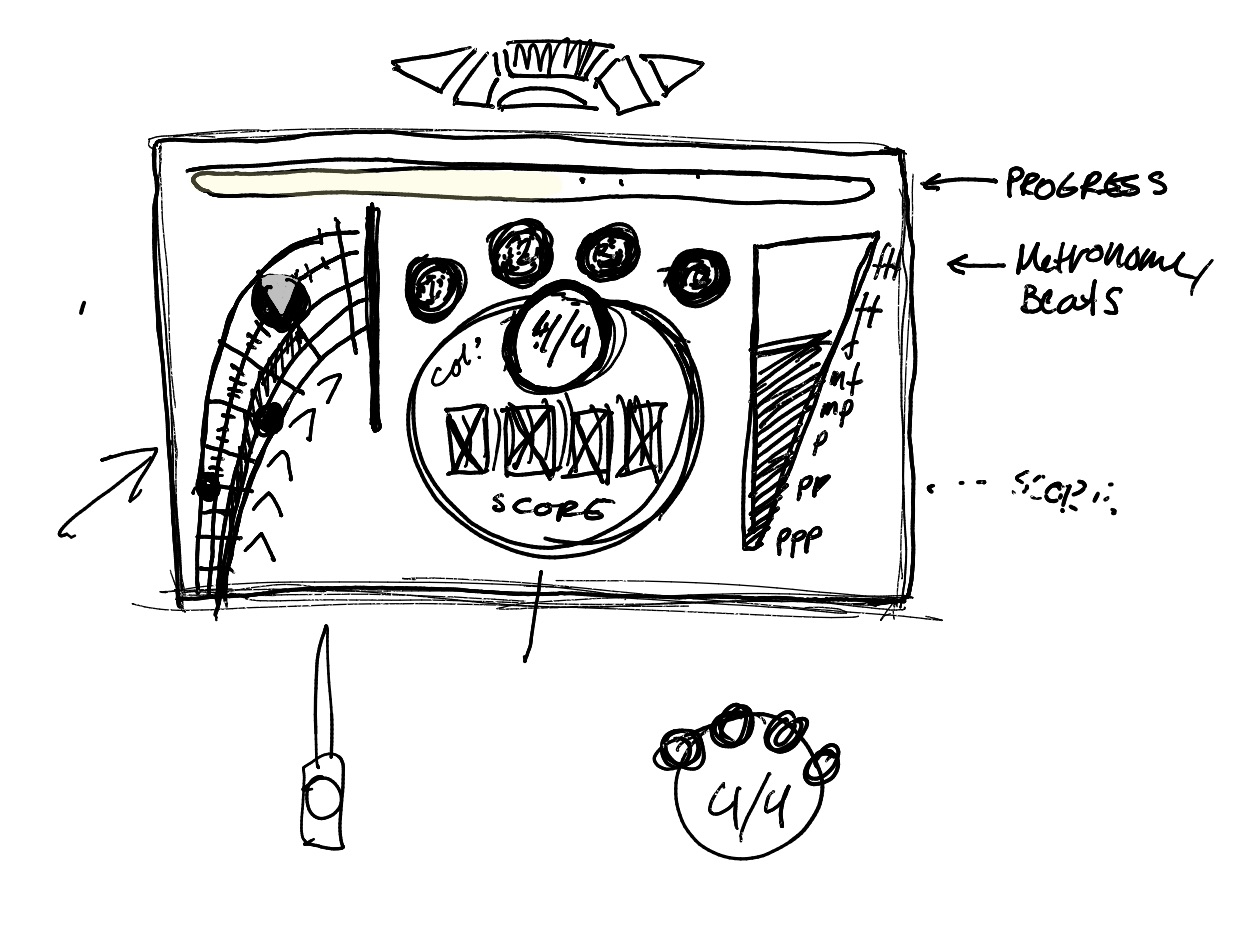
\includegraphics[width=0.75\textwidth]{images/sketch.jpg}
    \caption[Example sketch of the Conductor Table]{An initial concept sketch from the development of the Conductor Table.}
    \label{fig:tablesketch}
\end{figure}

\section{Interview}
After choosing to develop a conducting game, we interviewed a professional conductor over Skype to learn more about his experience of conducting and conductor training. The purpose of the interview was to better understand the different aspects of conducting. We also wanted to explore possibilities of involving VR games to promote the positive sides of conducting and to make any negative sides of the training process seem more engaging. During the interview, we found one motivation for the role of conducting, which is the feeling of control and leadership, as the orchestra follows your directions. It is relatively hard to get access to a whole orchestra for conducting training in real life, especially for conducting fanciers or novices. However, in a VR environment, it is possible to have access to a virtual orchestra with a customized composition at any time as long as the player has access to a VR device. With the interactions and feedback from the virtual orchestra, players can achieve greater motivation to keep on training. From the interview, we also got the idea that using unique virtual environments and game elements may ease the feeling of dullness and stress during repeated training. The feedback from the conducting expert confirmed pre-existing assumptions for the features in the conductor game and helped us to have a clearer vision about potential users.

\section{Tools}
The game was created using the Unity engine (version 2017.3.0.3f) with C\# as a language for the scripting components. Microsoft's Visual Studio 2017 Community was used as the Integrated Development Environment. Version control was done through Git using Github as our hosting service. Google drive was used for storing sound files, as these came close exceeding Github’s restrictions on file size, and to a large extent slowed the system down.
Valve’s Unity SteamVR plugin was used for communicating with the HTC Vive. Blender was used for modeling 3D assets, like the instruments and game world. The UI for the conducting table was created with Adobe Illustrator and Adobe Photoshop. The soundtrack used for the game was composed in Guitar Pro 5. Cubase 5 was used as the Digital Audio Workstation when generating audio from the midi tracks exported from Guitar Pro 5, using Virtual Studio Technology instruments from EastWest/Quantum Leap symphonic orchestra to produce the desired individual instrument tracks. Discord was used for intragroup communication.


\section{Development Methodologies}
The development followed a mixed methodology model with a focus on aspects that would allow us to work in parallel and quickly prototype features. Code hygiene factors was a low priority due to the limited time and we did not expect that performance would be an issue with such a limited game. We, therefore, adopted a ''critical path coding''~\cite{critical_path_coding} approach to get as much done with as little code as possible.

Developers usually worked individually after short discussions on architecture, however, pair programming techniques were employed for more challenging or unfamiliar problems. 
We originally intended to have a focus on the process, making proper use of issue tracking, branching strategies, and code reviews. However, early in the project, we came to the conclusion that this added unnecessary overhead to a time-limited project. We decided it would be more beneficial for the project that we spent more time on implementation rather than documentation and process.

In terms of meetings, we employed daily three minute meetings during the morning of every village day in a similar vein to those used in agile software methodologies. These meetings consisted of every group member mentioning any additional progress that had happened since the last day, what they planned to work on during the village day and discussing any potential problems that may arise. We kept these meetings to a maximum of three minutes per group member as a means to avoid situations where certain group members could end up dominating the discussions.
\chapter{Results} \label{chap:results}

\section{Game Design Document}
We generated an initial design document for the game, giving a brief overview of the envisioned game, and a plan for the game mechanics. This document can be found in the Appendix \ref{chap:appendix}.

\section{Game Implementation}
After creating the game design document we implemented a functional prototype of the conductor hero game. The source code and binaries are located on github\footnote{\url{https://github.com/Per-Morten/imt4310_conductor_hero}}. In order to play the game, a functioning HTC Vive headset is required. Instructions on how to install and play the game can be found on the main GitHub repository page. A youtube video\footnote{\url{https://www.youtube.com/watch?v=YQQTDyfQb-Q}} was recorded to demonstrate the features of the game.

\subsection{Asset Attribution}
The majority of assets used in Conductor Hero were created by us with a few exceptions:
\begin{itemize}
\item Particle Fog textures were acquired from Unity’s Standard Assets.
\item The skybox used in the game was acquired from the Unity Asset Store\footnote{\url{ https://assetstore.unity.com/packages/2d/textures-materials/sky/10-skyboxes-pack-day-night-32236}}   
\item The models for the HTC Vive Controllers were provided with the SteamVR plugin. 
\item The font used in the Conductor Table was acquired from dafont\footnote{\url{ https://www.dafont.com/white-rabbit.font}}. 
\end{itemize}

\subsection{Core Game Components}
The four core components that make up the game are: GameManager, Metronome, AudioManager, and MotionTracker.

The GameManager component manages musical cues as well as scoring. The Metronome component handles the core beat logic. It allows outside components to ask how close they are to being on beat. Other components can also add callbacks to the metronome which will be called every beat. The default sound for the metronome was removed, partly due to uncertainties regarding licensing. The AudioManager manages simultaneous playback of the multiple instrument tracks, metadata about song length and supports muting and unmuting individual tracks. 

Finally, the MotionTracker component handles game logic related to the right hand conducting. This includes managing the visuals of the pattern and any logic for tracking the player’s movement within the pattern, using the tracking spheres in the scene.  

\subsection{Standard game flow} 
The following section describes the standard game flow in the prototype level of Conductor Hero:
\begin{itemize}
\item The player starts the game and the stage will go to an unlit state.  
\item The two controllers are separated by having one with a laser pointer and one without. The “laser pointer” on one of the controllers indicates that it should be held in the left hand.
\item In order to start the game, the player needs to hold their right controller in an upwards position where they would feel comfortable having the top of the conducting pattern and press the menu button to start. 
The game starts a countdown to the song which ends with the first cue.
\item While playing, the player’s left hand is used to hit cues on beat while their right hand is used to keep the conducting pattern going. 
    \begin{itemize}
    \item[--] A cue appears at designated times during the song. The cue has a circular progress bar which implies when the player is supposed to hit it.
    \end{itemize}
\item The game ends when the song is finished.
\end{itemize}

\subsection{Shortcomings of the Prototype}
In the prototype, the game will start the countdown to the song and show the pattern to the player, but currently, it will also start counting score for movement even if the song has not properly started yet. This is unintended as we would like to start measuring score after the first cue, but we did not have the time to fix this by the end of the project. The game is also supposed to end once the song duration has expired, but we do not have any additional end states to signify this due to time constraints.  

\subsection{Playtesting}
As part of the development, we performed a lot of internal testing within the development team. We also had an initial playtesting session with the entire group and also asked some members of other teams to try out the game and give feedback. This playtesting session is further discussed in the Discussion Chapter.

\section{Presentation}
As part of the course, we also had a presentation towards the end where we showed off the project to the class, the supervisor and industry externals. The slides from the presentation can be found on Google Slides~\footnote{\url{https://docs.google.com/presentation/d/1unr5goORWJpajkHhiNFVHJUfyByFeLB_AzXME653Kd0/edit?usp=sharing}}
\chapter{Implementation}
\section{Implementation Details and Encountered Challenges}
\subsection{Beat Logic}
Since the game relies heavily on fixed beats that correspond to the music, we decided to create a central metronome object. The metronome ended up supporting two ways of identifying the current beat, a beatID property returning the current beat, and a callback called on each beat update. All game objects were originally intended to register as listeners to the ''OnBeatTickCallback''. However, as we were not in total control over the order of callback executions, we ran into logical inconsistencies in the cueing system. We worked around this issue by only registering callbacks in order independent systems. During these callbacks, each system would be responsible for updating their order dependent subsystems through direct function calls. This introduces some more coupling into the codebase, but not to an unmanageable degree. 

\subsection{Audio Playback}
Requiring the player to cue in different instruments throughout a song, un-muting individual instruments on success or muting them on failure, presented an interesting challenge. Controlling the different tracks was done through a simple enum, however, we ran into issues that the tracks were not necessarily synchronized, which was devastating to the game. Luckily Unity’s AudioSource supports scheduling tracks, fixing the synchronization problem~\cite{unity_audio_source_api}. 

\subsection{Cues}
\begin{figure}[tbph]
    \centering
    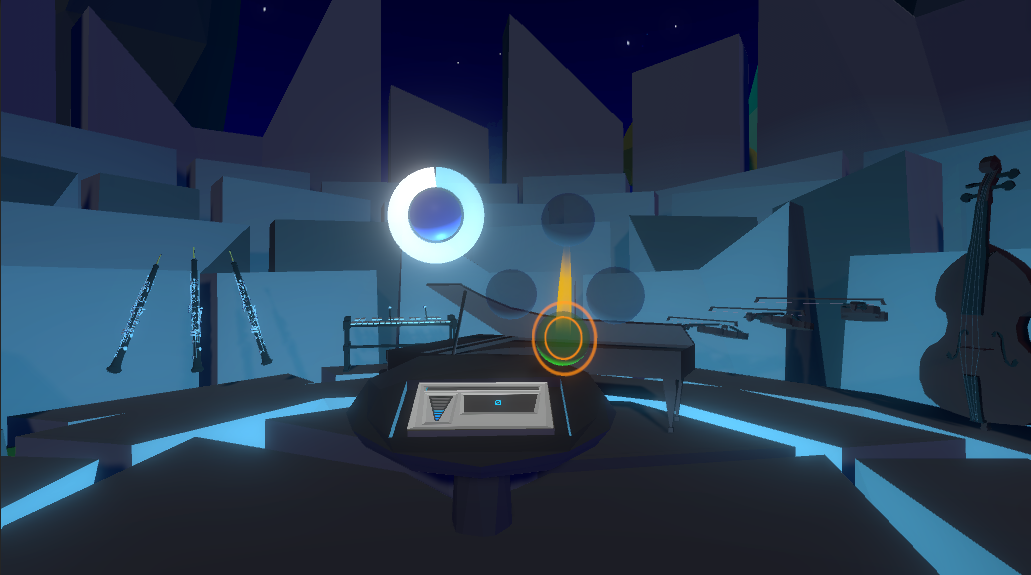
\includegraphics[width=1.0\textwidth]{images/cue}
    \caption[Screenshot of a Cue]{This screenshot shows a Cue that is ready to be hit by the player to signify that an instrument track should start playing.}
    \label{fig:cue}
\end{figure}

The musical cues were implemented as a finite state machine as seen in Figure~\ref{fig:cue_fsm}. The cue transitions between different states are based on the number of beats left before the instrument should enter and whether or not it has been hit by the player. Implementing the cues as a finite state machine allowed us to structure the code in a way that was consistent with the state transitions of the cue, making it easy to follow the logical execution of the cue behavior. 
An alternative solution could be to go with a full state pattern\cite{game_programming_patterns}, with separate classes for each state. However, we did not deem the cue logic to be complex enough to justify such a solution. An example of a cue can be seen in Figure~\ref{fig:cue}.

\begin{figure}[tbph]
    \centering
    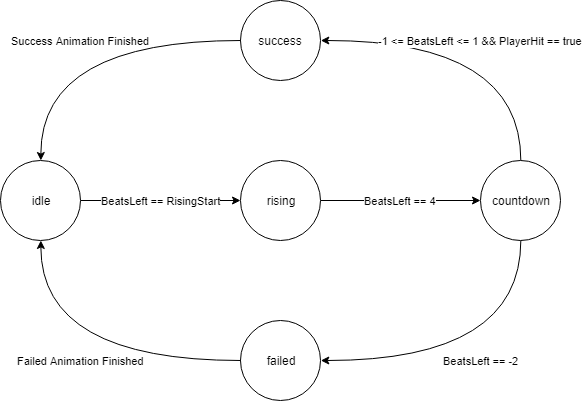
\includegraphics[width=1.0\textwidth]{images/cue_fsm}
    \caption[Cue Finite State Machine]{This model shows the finite state machine used for the cueing logic}
    \label{fig:cue_fsm}
\end{figure}

\subsection{Creating an illusion of glowing light for objects without light sources}
In terms of the in-game environment, the original plan was to include bright glowing mushrooms scattered around the area. A problem arose when the number of illuminated mushrooms in the scene exceeded a manageable amount, severely reducing the performance of the application. We wanted to keep the visual integrity of the scene as close as possible to its original Blender model, so we came up a workaround for the problem.

Instead of illuminating the mushrooms, we worked around the issue by changing their material to a bright colour. We then added a bloom post-processing effect, creating an illusion of glowing light around the mushrooms. This did not light up the scene in any way, but the small size of the mushrooms and the sheer amount of them made this the most logical solution to keep the visuals intact without sacrificing performance. 

\subsection{Creating simple fog effects using Unity's particle system}
\begin{figure}[tbph]
    \centering
    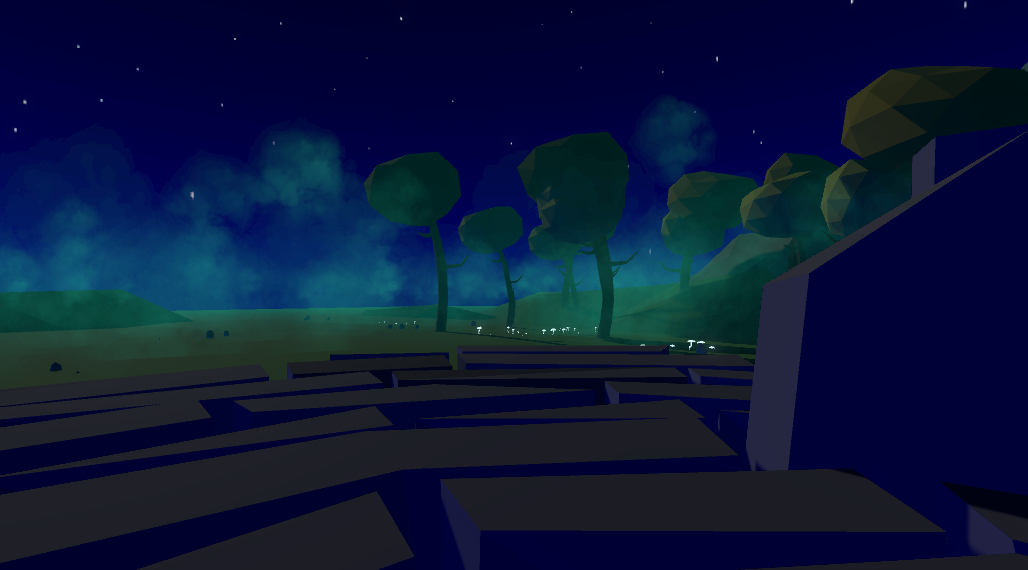
\includegraphics[width=1.0\textwidth]{images/fog}
    \caption[Screenshot of ingame fog]{This screenshot showcases how the ingame fog looks like.}
    \label{fig:fog}
\end{figure}
The original concept idea for the in-game environment also included some green fog that was spread around in the scene. Ideally, this could be handled through the use of Volumetric Fog or similar implementations, but due to limited time to work on the project, we had to find a quicker and simpler solution to implement while still providing a relatively good approximation of the fog effect. 

We implemented fog using Unity's Particle System component, utilizing a single fog texture from the Unity particle effects standard assets pack. We then layered several particle systems on top of each other with small variations in settings like particle size, rotation, lifetime, and, emission rate to create the illusion of fog. We combined this with Unity’s distance fog functionality which makes geometry fade towards a gradient colour based on distance from the camera. This enhances the illusion of fog. The end result does not look equivalent to Volumetric Fog, but we believe it serves its purpose, and saved us a good amount of development resources. A screenshot illustrating the visuals of the fog can be seen in Figure~\ref{fig:fog}. 


\subsection{Demonstrating the conducting pattern visually}
\begin{figure}[tbph]
    \centering
    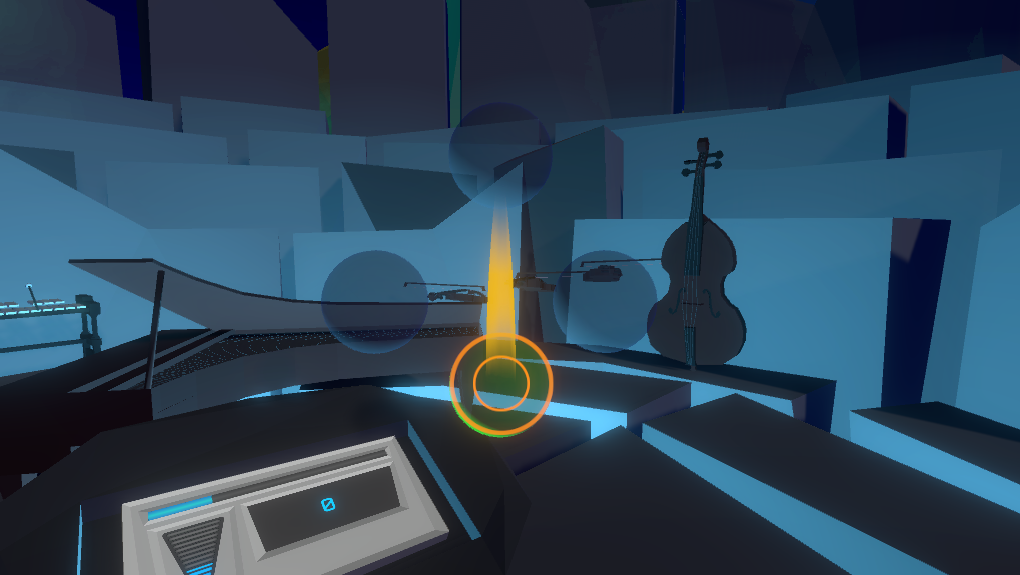
\includegraphics[width=1.0\textwidth]{images/spheres-trail-pulse}
    \caption[Screenshot of Motion Tracking Spheres]{This screenshot illustrates the four motion tracking spheres used for conducting. The currently active sphere is coloured green with expanding circles emmitting at the start of the beat. There is also a trail that further illustrates how the player should move their hand between beats.}
    \label{fig:trackingspheres}
\end{figure}
The initial implementation for demonstrating the conducting pattern included four transparent spheres. These spheres would change their material from a gray to a green colour, indicating that the player was supposed to touch it at that beat. This method made it possible to see the conducting pattern as only one sphere would be green at any given time, and the colour changed on beat which reinforced the rhythmic movement to the player. While the initial implementation was fine for internal testing, later playtesting with externals provided some insight into the fact that more visual feedback and information would be preferred. This was particularly apparent for testers with no prior experience in conducting as they did not understand how they were supposed to move their hands. 

Our solution to this was to create trails between the four different spheres which demonstrated the pattern in a slightly more visual manner. 
This was handled by taking an invisible ''GameObject'' with a ''TrailRenderer'' and interpolate it between the previous beat's sphere and the next beat’s sphere.

To emphasize the rhythm we added expanding circles instantiated on the beat. These also indicated the next step in the conducting pattern. Additionally, the first beat was emphasized with a different colour to more easily allow the player to get back into the rhythm. This can be seen in Figure~\ref{fig:trackingspheres}. 

If more time was available, we would probably have used Bezier curves to demonstrate the conducting pattern in a more correct manner rather than having linear trails between the spheres. The added complexity of this approach is negligible, but it would take a fair amount of time to create proper looking curves without any visual aids in the Unity editor for bezier curve control. 


\subsection{Binding animation states to the beat}
To emphasize the rhythm of the song in Conductor Hero we ended up tying the majority of animation states to the ''OnBeatTickCallback'' in the Metronome component. While this was an interesting way to work with animations it also posed a fair share of problems. An issue with changing animation states on beat was the cases where it would be preferable to change the animation at different times than the callback. An example of this issue is detailed below: 

The player is supposed to start moving their hand towards the next beat before it starts, but the interpolated trail only starts moving towards the next sphere whenever the next beat triggers the beat callback. With a linear interpolation, this means that the trail lags behind where the player should have moved their hand between two beats, potentially confusing the player and making it hard to read the rhythm from the movement of the trail. To work around this we slightly modified the linear interpolation by parameterizing the input time through the use of an ''AnimationCurve''. This makes it possible to control the velocity of the animation throughout its lifetime. Using this, we made the velocity of the trail very fast early on, to create a more natural motion towards its destination to where the player needs to move their hand. 


\subsection{Providing Visual Player Feedback}
\begin{figure}[tbph]
    \centering
    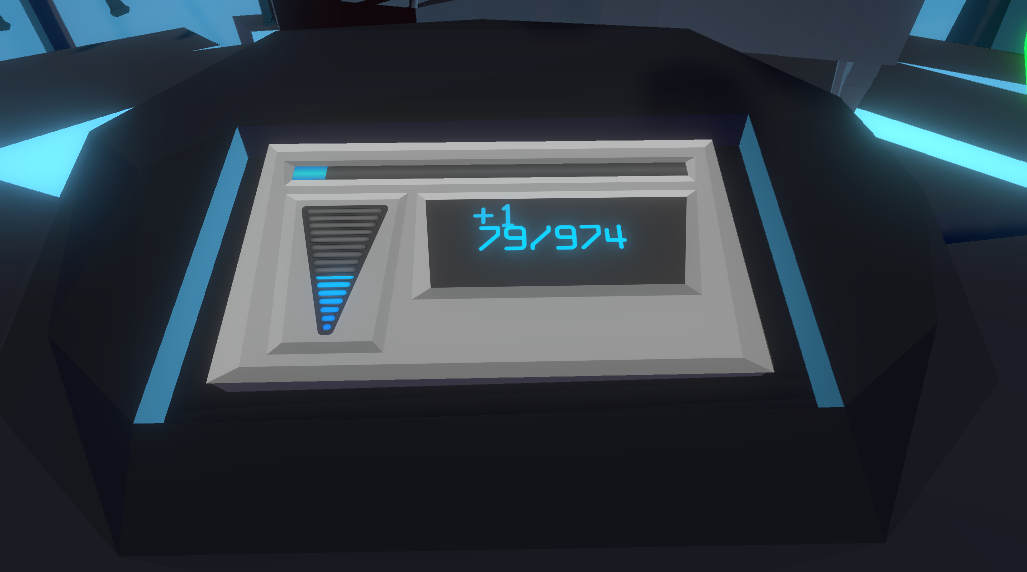
\includegraphics[width=1.0\textwidth]{images/scorePopup}
    \caption[Screenshot of the Conductor Table Dashboard]{This screenshot shows the dashboard on the Conductor Table where the top bar is current song progress, the left bar is the volume bar and the display on the right shows current score compared to maximum score.}
    \label{fig:table}
\end{figure}

It is important to provide the player with enough visual feedback for them to understand how their actions are being reflected in the game. In Conductor Hero, visual feedback is provided using several methods. 

Particle effects in the tracking spheres indicate whether or not the player is conducting correctly. Red particles indicate that the player is off beat, while green signifies being on beat.

We are also providing some visual feedback on the conductor table whenever the player gains score for either conducting on beat or hitting cues. 

A small popup appears in the table’s canvas whenever the score is increased, telling the player how much score their actions have resulted in. A score of ''+10'' is given for hitting cues correctly while a score of ''+1'' is given for every conducting motion that is on beat. The score values obtained by hitting cues could have been bigger, and more visually distinct, to further emphasize the larger amount of points gained, but we did not implement this due to time constraints. The visual feedback used in the conductor table can be seen in Figure~\ref{fig:table}.

\subsection{Design of the in-game environment}
\begin{figure}[tbph]
    \centering
    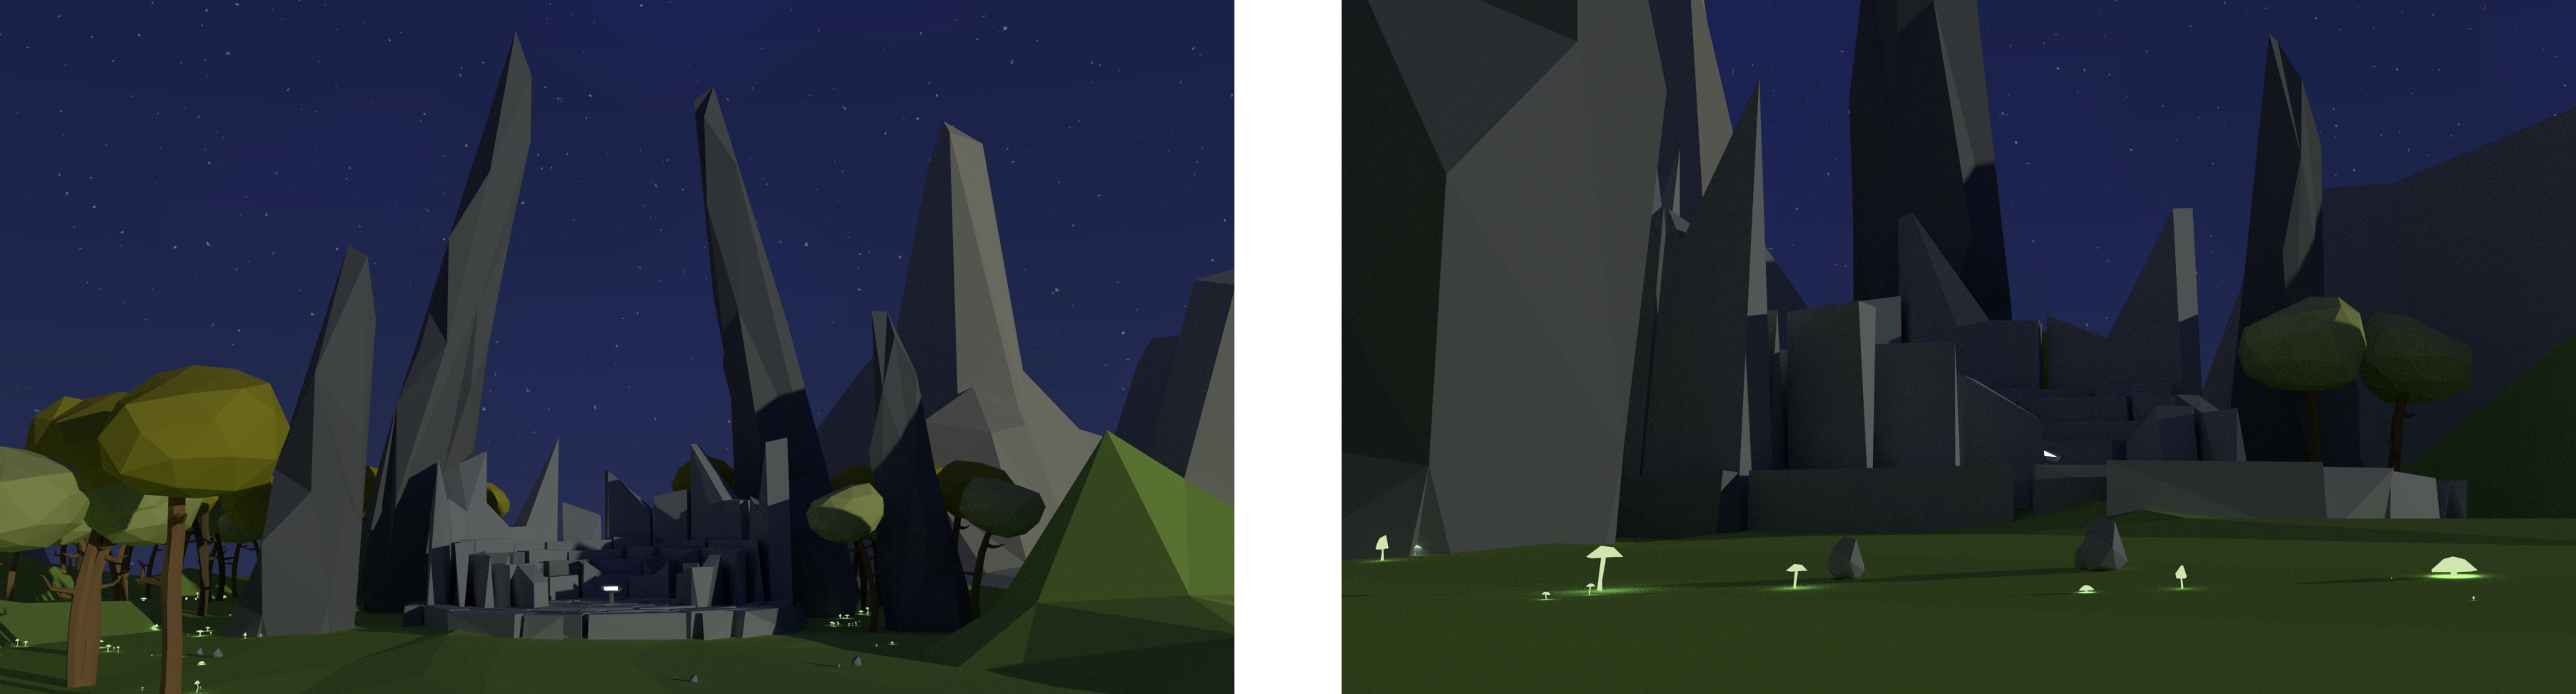
\includegraphics[width=1.0\textwidth]{images/Forest}
    \caption[The forest scene from the prototype]{These screenshots showcase the 3D environment made in Blender.}
    \label{fig:Forest}
\end{figure}

\begin{figure}[tbph]
    \centering
    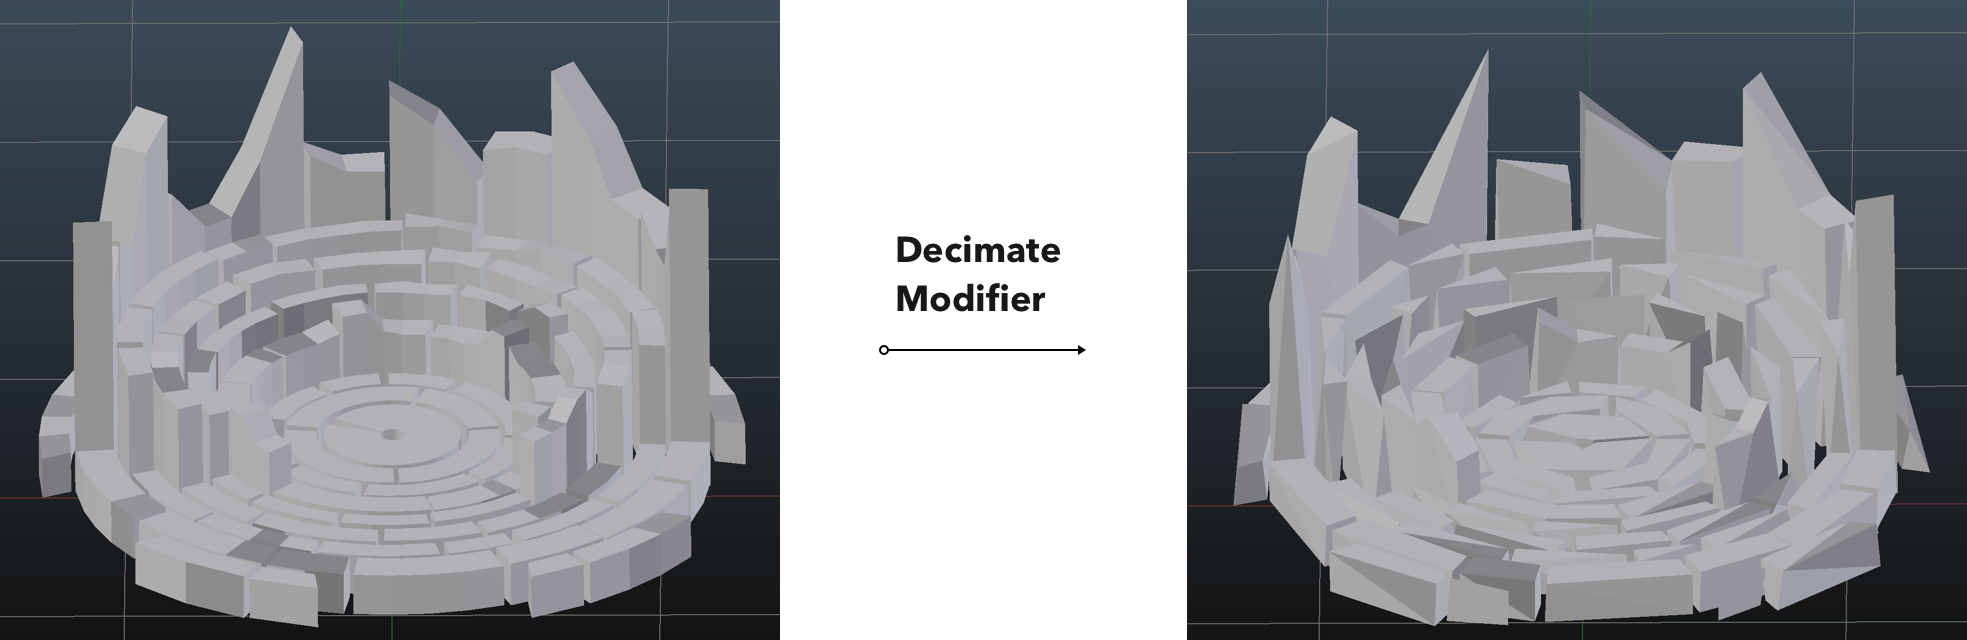
\includegraphics[width=1.0\textwidth]{images/lowPolyDecimate}
    \caption[Example use of the Decimate Modifier in Blender]{This figure illustrates how the Decimate Modifier in Blender can create a low poly version of a regular 3D model.}
    \label{fig:lowpolydecimate}
\end{figure}


A goal of Conductor Hero was to immerse the players into a unique VR environment while conducting the orchestra. We discussed various environments like a seabed, or the outer space, but settled on the forest scene for the prototype due to time constraints. We envisioned that the musicians of the orchestra could change to fit the environment, turning into beasts, fish, or aliens. The game has a low poly style, as the concept did not require high-fidelity graphics. We believe that the visuals look appealing to the audiences while being stylish, they are easy to create and iterate upon, which has the added benefit of fitting within the time scope of our project. To achieve this style we used the Decimate modifier in Blender to decrease the number of polygons in each object. An example of how the modifier was used can be seen in Figure~\ref{fig:lowpolydecimate} while the final 3D model of the environment can be seen in Figure~\ref{fig:Forest}. We reviewed existing games using low poly styles and imagery of forests to create a harmonious colour palette for our scene. The colour palette we ended up using is shown in Figure~\ref{fig:colourpalette}. During this review, we found that many existing rhythm games use lighting to emphasize the rhythmic feel of the song. To achieve the same effect we introduced lighting into the floor that the player is standing on, which pulsates with the rhythm. The cyan light below the stage and the ''glowing'' mushrooms around the environment further enhance the fantasy theme of the scene.

\begin{figure}[H]
\centering
    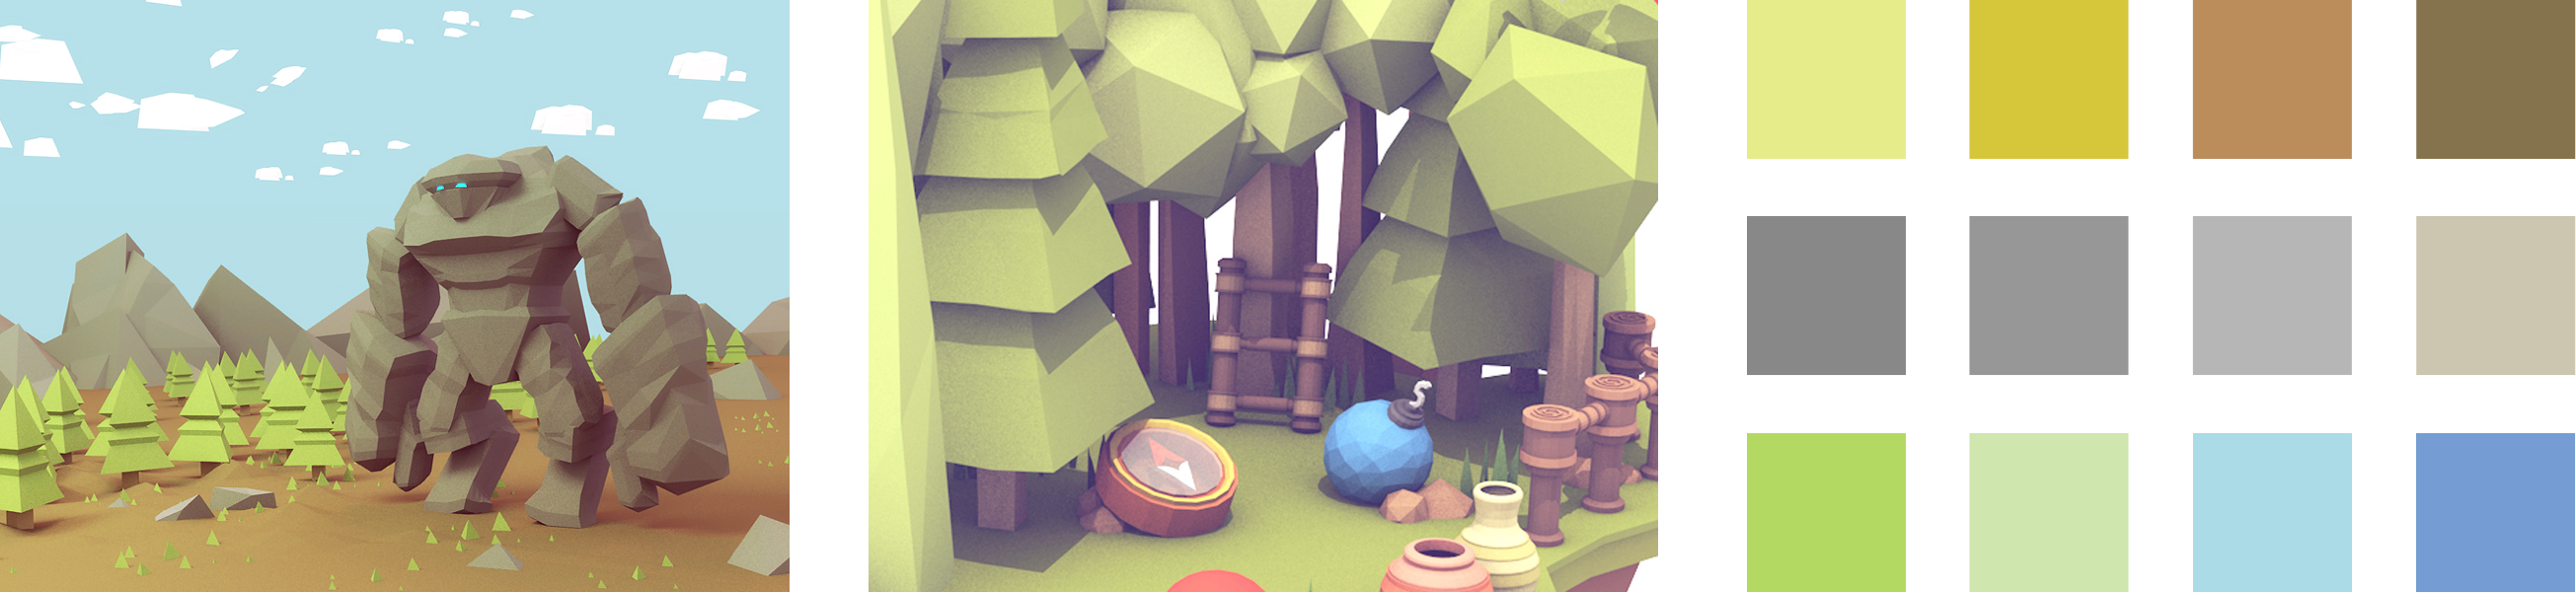
\includegraphics[width=1.0\textwidth]{images/sceneColourPalette}
    \caption[The colour palette for the ingame scene]{The colour palette we used in the project was influenced by styles similarly to what is illustrated here. The final colour palette is seen on the right. }
    \label{fig:colourpalette}
\end{figure}
\chapter{Discussion} \label{chap:discussion}

\chapter{Conclusion}
\chapter{Future Work}

While we managed to get further than we had expected, there is still a lot of work left unfinished. Time constraints was a challenge throughout the project, and we believe that the finished product could be significantly improved with further testing. With more time available, user testing and user experience (UX) design would have been a priority for the group.  User feedback can be an invaluable resource during the development of a product, and we believe that it would be beneficial to make this a priority in the possible further development of Conductor Hero. 

Turning the prototype into a fully fledged game would require a complete rewrite of most of the game systems, to create more generalized and reusable solutions. However, this rewrite would be necessary to achieve other desirable features, like more levels, songs, and the potential for user-generated content. A fully fledged game would also require us to design a complete user interface for the user to interact with, which would present us with more challenges in the VR space. 

During the initial design phase, we came up with several ideas for extending the mechanics of the game, for example, a level where you don’t just conduct the instruments but also the virtual environment, creating a visual experience that reinforced the feeling of the music. To keep the scope and mechanics at a manageable level these ideas were not pursued, however, we would like to explore these ideas in an extended project.



\bibliographystyle{ntnuthesis/ntnubachelorthesis}
\bibliography{inc/ref}

\appendix 
%after this line all chapters will have letters instead of numbers
% spreadsheet data?
\chapter{Appendix} \label{chap:appendix}
\section{Game Design Document}

\subsection{What is “Conductor Hero”?}
Conductor Hero is a VR conducting game that allows the player to take the role of a conductor as the name implies and conduct a band/orchestra of instruments to given music tracks. We have taken inspiration from games like Guitar Hero™ where the focus of the game is not necessarily to be authentic to real life experience, but rather provide an approximation and highlight the experience of conducting instead. 

\subsection{Planned Game Functionality}
Our initial plan for the game includes several different functionalities. First off, we plan to have two different types of game modes. Freestyle mode is where the player can freely cue instruments in and out as they wish where the cueing itself is not scored. Performance mode on the other hand requires the player to cue in instruments at specific points in the music track. In Performance mode we would also like to score the cueing according to how close to correctness it is in relation to timing. 

The band/orchestra will include several instruments. This should include violins, violas, contrabass, harpsichord, glockenspiel and oboes. 

In terms of conducting the player can use their dominant hand to conduct the music with a time signature of 4/4 for the minimum viable product. The other hand can then be used to cue in groups of instruments. The player is scored depending on how close their conducting movements are to being correct and how rhythmically correct it is. We want to be very lenient on the movement itself as it is hard to expect perfect conducting motions every time and rather focus on scoring the rhythmic aspect. At the same time it should not be possible to cheat the conducting pattern. The nondominant hand could also potentially be used to control the intensity of instruments. By doing so we can for example have three different instrument intensities and allow the player to switch between them with the nondominant hand.

Within the game we also want to have a Conductor Table/Dashboard that contains all relevant UI elements. The list of what we want to display on this screen is as follows: Score, communication on where to cue instruments in, duration left on song and current song volume. 

\subsection{Project Scope} 
For this project, we plan to scope for a minimum viable product containing only one level as we have a limited amount of development time. If the MVP milestone is met early then we can also potentially add the ability to share the player’s performance from freestyle mode as a performance mode challenge. 


\end{document}
